\documentclass{setupFiles/final_exam_sust}

%%%%%%%%%%%%%%%%%%%%%%%%%%%%%%%%%%%%%%%%%%%%%%%%%%%%%%%%%%%
%%%%% About printing the solution and Table of Specifications (TOS)

% \printanswers   %% Uncomment this if you want to print the solution
 \printTOStrue   %% Uncomment this to include the TOS page at the end [3]

%%%%%%%%%%%%%%%%%%%%%%%%%%%%%%%%%%%%%%%%%%%%%%%%%%%%%%%%%%%%%%%%%%%%%%%%%%%%%%%%%%%%%%%
%%%%%%%%%%%%%%%%%%%%%%%%%%%%%%%%%%%%%%%%%%%%%%%%%%%%%%%%%%%%%%%%%%%%%%%%%%%%%%%%%%%%%%%
%%%%% Define all exam variables (Adapt this part for you)

\newcommand{\institutionName}{Shahjalal University of Science and Technology}
\newcommand{\institutionNameShort}{SUST}
\newcommand{\deptName}{Department of Electrical and Electronic Engineering}
\newcommand{\deptNameShort}{EEE}


\newcommand{\examName}{B.Sc. (Engg.) First Year, First Semester Final Examination-2022}
\newcommand{\courseCode}{EEE~0713~1121}
\newcommand{\courseTitle}{Course Title For This Course Code}
\newcommand{\SessionExaminee}{2020-2021}
\newcommand{\totalMarks}{60}
\newcommand{\totalCredits}{3.0}
\newcommand{\examDuration}{3~Hours}


\newcommand{\examDate}{March~08,~2019~--~9:30} % Exam date and time or the questing writing date and time

%\newcommand{\examDate}{\DTMnow} % Today's date and current time


\newcommand{\specialInstruction}{Answer \textbf{all} the questions}



\newcommand{\teacherName}{Name of question setter}
\newcommand{\teacherUniqueID}{N07R28S33}

%%%%%%%%%%%%%%%%%%%%%%%%%%%%%%%%%%%%%%%%%%%%%%%%%%%%%%%%%%%%%%%%%%%%%%%%%%%%%%%%%%%%%%%
% Setup the internal switch for conditional TOS processing
\makeatletter
\@ifundefined{ifprintTOS}{\newif\ifprintTOS}{}
\makeatother
%%%%%%%%%%%%%%%%%%%%%%%%%%%%%%%%%%%%%%%%%%%%%%%%%%%%%%%%%%%%%%%%%%%%%%%%%%%%%%%%%%%%%%%
\begin{document}

%%%%%%%%%%%%%%%%%%%%%%%%%%%% The Header of the question %%%%%%%%%%%%%%%%%%%%%%%%%%%%%%%
\input{TexFiles/examHeader}

%%%%%%%%%%%%%%% Part-A %%%%%%%%%%%%%%%%%%%%%%%%%%%%%%%%%%%%%%%%%%%%%%%%%
\begin{center}
    \textbf{\large {Part-A}}\\
     \textit{[\specialInstruction{}]}
\end{center}

%%%%%%%%%%%%%%%%%%%%%%%%%%%%%%%%%%%%%%%%%%%%%%%%%%%%%%%%%%%%%%%%%%%%%%%%

\begin{questions}
	


\input{TexFiles/Q1}  	 
%%%%%%%%%%%%%%%%%%%%%%%%%%%%%%%%%%%%%%%%%%%%%%%%%%%%%%%%%%
%%%%%%%%%%%%%%%%%%%%%%  Question#01  %%%%%%%%%%%%%%%%%%%%%
%%%%%%%%%%%%%%%%%%%%%%%%%%%%%%%%%%%%%%%%%%%%%%%%%%%%%%%%%%
\begin{comment}
  Put all the topics for this question.
\end{comment}
%%%%%%%%%%%%%%%%%%%%%%%%%%%%%%%%%%%%%%%%%%%%%%%%%%%%%%%%%%
\question 
\begin{parts}
%%%%%%%%%%%%%%%%%%%%%%%%%%%%%%%%%%%%%%%%%%%%%%%%%%%%%%%%%%	
\part[2] For units, you can use SI units; \textcolor{blue}{for example}, \textcolor{red}{\qty{2}{\micro\meter}} can be achieved by using the command \verb|\qty{2}{\micro\meter}| or \verb|\SI{2}{\micro\meter}|. This type \verb|\qty{2}{\micro\meter}| is the modern standard in \textcolor{red}{\texttt{siunitx} v3}, while \verb|\SI{2}{\micro\meter}| is the legacy syntax from older versions.



\part[1] In case you need to use the unit for an expression \textcolor{blue}{as for example} \textcolor{red}{ \(20sin(\omega t)\)~\si{\milli\ampere}}, right after the expression, you can use the command \verb|\si{\milli\ampere}|.


\begin{solution}

\end{solution}
%%%%%%%%%%%%%%%%%%%%%%%%%%%%%%%%%%%%%%%%%%%%%%%%%%%%%%%%%%
\part[4] Two resistors of values \qty{1}{\kilo\ohm} and \qty{4}{\kilo\ohm} are connected in series across a constant voltage supply of \qty{100}{\volt}. A voltmeter having an internal resistance of \qty{12}{\kilo\ohm} is connected across the \qty{4}{\kilo\ohm} resistor. Draw the circuit and calculate: 

\begin{subparts}
		\subpart True voltage across \qty{4}{\kilo\ohm} resistor before the voltmeter was connected.
		\subpart Actual voltage across \qty{4}{\kilo\ohm} resistor after the voltmeter is connected and voltage recorded by the voltmeter.
	\end{subparts}



\begin{solution}

\end{solution}
%%%%%%%%%%%%%%%%%%%%%%%%%%%%%%%%%%%%%%%%%%%%%%%%%%%%%%%%%%	
\part[5] \color{red}Figure(pdf, png, etc) can be inserted using the \verb|\includegraphics{nameOfFigure}| command as shown below. : \color{black}Find the rms value of the current waveform of Fig.\ref{fig:currentWaveform}. If the current flows through a \qty{9}{\ohm} resistor, calculate the average power absorbed by the resistor. 


		\begin{figure}[H]
			 \centering 
			 \includegraphics[width=0.30\textwidth]{Fig11.15_ElectricCircuit_SadikuPg446_3E}
			 \caption{}
             \label{fig:currentWaveform}
        \end{figure}
		


\begin{solution}

\end{solution}
%%%%%%%%%%%%%%%%%%%%%%%%%%%%%%%%%%%%%%%%%%%%%%%%%%%%%%%%%%			
\end{parts}

  	
\input{TexFiles/Q3}  	




\begin{center}
\textbf{OR}\\[6pt]
\end{center}	

\input{TexFiles/Q3OR}	

%%%%%%%%%%%%%% Part-B %%%%%%%%%%%%%%%%%%%%%%%%%%%%%%%%%%%%%%%%%%%%%%%%%%%%%%%%%%
% \newpage
%\pagebreak

\begin{center}
    \textbf{\large {Part-B}}\\
     \textit{[\specialInstruction{}]}
\end{center}
%%%%%%%%%%%%%%%%%%%%%%%%%%%%%%%%%%%%%%%%%%%%%%%%%%%%%%%%%%%%%%%%%%%%%%%%%%%%%%%%%%%%%%%%%%%%%%%%%%%%%
%%%%%%%%%%%%%%%%%%%%%%%%%%%%%%%%%%%%%%%%%%%%%%%%%%%%%%%%%%%%%%%%%%%%%%%%%%%%%%%%%%%%%%%%%%%%%%%%%%%%%
%%%%%%%%%%%%%%%PART-B(Question#04--> 
%%%%%%%%%%%%%%%%%%%%%%%%%%%%%%%%%%%%%%%%%%%%%%%%%%%%%%%%%%%%%%%
%%%%%%%%%%%%%%%%%%%%%%%%%%%%%%%%%%%%%%%%%%%%%%%%%%%%%%%%%%%%%%%%%%%%%%%%%%%%%%%%	
\question 
\begin{parts} 
%%%%%%%%%%%%%%%%%%%%%%%%%%%%%%%%%%%%%%%%%%%%%%%%%%%%%%%%%%%%%%%%%	
\part[6] An Inverse Definite Minimum Time (IDMT) overcurrent relay is connected to a \qty[parse-numbers=false]{400/5}{\ampere} Current Transformer (CT) with a Plug Setting (PS) of $125\%$. The characteristic curve for $\text{TMS} = 1.0$ is shown in Fig.~\ref{fig:graph}. If a symmetrical fault current of \qty{5000}{\ampere} flows through the primary side, calculate:

\begin{subparts}
    \subpart The Plug Setting Multiplier ($\text{PSM}$) of the relay.
    \subpart The operating time of the relay for $\text{TMS} = 0.4$.
    \subpart The required $\text{TMS}$ setting if the relay must operate in $1.8\text{ seconds}$.
\end{subparts}


\begin{figure}[H]
\centering
\resizebox{0.5\textwidth}{!}{% Adjust width (e.g., 0.6\textwidth, 10cm, etc.) as needed
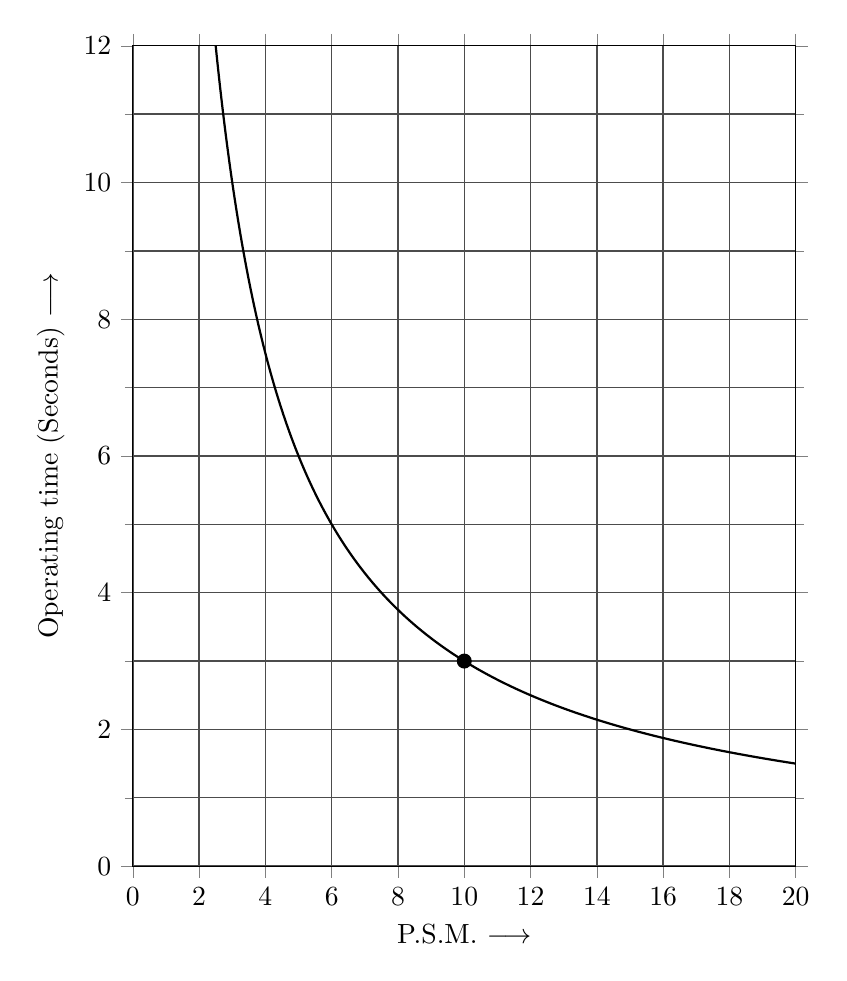
\begin{tikzpicture}
\begin{axis}[
    width=10cm,
    height=12cm,
    xmin=0, xmax=20,
    ymin=0, ymax=12,
    % Horizontal labels at 0, 2, 4... 20
    xtick={0,2,4,6,8,10,12,14,16,18,20},
    % Vertical labels at 0, 2, 4... 12
    ytick={0,2,4,6,8,10,12},
    % NO extra vertical lines (only at the 2-unit marks)
    minor x tick num=0,
    % EXTRA horizontal lines (adds 1 line between the 2-unit marks)
    minor y tick num=1,
    % Grid settings
    grid=both,
    % Make all grid lines look the same to match the photo
    grid style={line width=0.5pt, draw=black!70},
    % Axis labels
    xlabel={P.S.M. $\longrightarrow$},
    ylabel={Operating time (Seconds) $\longrightarrow$},
    % Visual formatting
    tick align=outside,
    axis lines=box,
    enlargelimits=false,
    samples=200
]

% The IDMT characteristic curve function
\addplot[
    domain=2.1:20, 
    smooth, 
    thick, 
    black
] {30/x}; 

% The dot at PSM=10, Time=3
\addplot[only marks, mark=*, mark size=2.5pt] coordinates {(10,3)};

\end{axis}
\end{tikzpicture}%
}
\caption{IDMT Overcurrent Relay Characteristic Curve}
\label{fig:graph}
\end{figure}



\begin{solution}
\textbf{(a) Plug Setting Multiplier ($\text{PSM}$):}
$$\text{Pick-up Current} = I_{\text{pickup}} = 5\text{ A} \times 1.25 = 6.25\text{ A}$$
$$\text{Secondary Fault Current} = I_{\text{sec}} = 5000\text{ A} \times \left(\frac{5}{400}\right) = 62.5\text{ A}$$
$$\text{PSM} = \frac{I_{\text{sec}}}{I_{\text{pickup}}} = \frac{62.5\text{ A}}{6.25\text{ A}} = 10$$

\textbf{(b) Operating time for $\text{TMS} = 0.4$:}
From Fig.~\ref{fig:graph}, at $\text{PSM} = 10$, the operating time at $\text{TMS} = 1.0$ is $t_{1.0} = 3.0\text{ s}$.
$$t = t_{1.0} \times \text{TMS} = 3.0\text{ s} \times 0.4 = 1.2\text{ s}$$

\textbf{(c) Required $\text{TMS}$ for $t = 1.8\text{ s}$:}
$$\text{TMS} = \frac{t}{t_{1.0}} = \frac{1.8\text{ s}}{3.0\text{ s}} = 0.6$$
\end{solution}
%%%%%%%%%%%%%%%%%%%%%%%%%%%%%%%%%%%%%%%%%%%%%%%%%%%%%%%%%%%%%%%%%		
\part[4]For the emitter bias network of Fig.~\ref{fig:ckt-bjt-emitter-bias} determine \(I_{B}\), \(I_{C}\), \(V_{CE}\), \(V_C\), \(V_E\) and \(V_B\).

\begin{figure}[H]
\centering
\resizebox{0.6\textwidth}{!}{% Adjust width (e.g., 0.6\textwidth, 10cm, etc.) as needed
\begin{tikzpicture}
	% Paths, nodes and wires:
	\draw node[npn] (N1) at (6, 4) {} node[anchor=west] at ([xshift=0.88cm]N1.east){$\beta = 50$};
	\draw (6, 7) to[american resistor, l={$2~k\Omega$}, label distance=0.02cm] (6, 4.77);
	\draw (5.16, 4) -- (2, 4);
	\draw (3, 7) to[american resistor, l_={$430~k\Omega$}, label distance=0.02cm] (3, 4);
	\draw (3, 7) -- (6, 7);
	\draw node[circ] at (4.51, 7) {};
	\draw (4.5, 7) -| (4.5, 7.5);
	\draw node[ocirc] (N2) at (4.5, 7.5) {} node[anchor=south] at (N2.north){$ +20~V$};
	\draw (7.316, 4.77) to[curved capacitor, l={$10~\mu F$}, label distance=0.02cm] (10.316, 4.8);
	\draw (2, 4) to[curved capacitor, l_={$10~\mu F$}, label distance=0.02cm] (0, 4);
	\draw node[ocirc] (N3) at (0, 4) {} node[anchor=east] at (N3.west){$v_i$};
	\draw node[ocirc] (N4) at (10.316, 4.8) {} node[anchor=west] at (N4.east){$v_o$};
	\draw (6, 4.77) -- (7.316, 4.77);
	\draw node[circ] at (3, 4) {};
	\draw node[circ, xscale=1.13, yscale=1.13] at (6, 4.77) {};
	\draw (6, 3.23) to[american resistor, l={$1~k\Omega$}, label distance=0.02cm] (6, 1);
	\draw (8, 2.5) to[capacitor, l={$40~\mu F$}, label distance=0.02cm] (8, 1);
	\draw (6, 3.23) -| (8, 2.5);
	\draw node[tlground] at (6, 1) {};
	\draw node[tlground] at (6, 1) {};
	\draw node[tlground] at (8, 1) {};
	\draw node[tlground] at (8, 1) {};
	\draw node[circ] at (6, 3.23) {};
\end{tikzpicture}
}
\caption{}
\label{fig:ckt-bjt-emitter-bias}

\end{figure}


\begin{solution}


\end{solution}
%%%%%%%%%%%%%%%%%%%%%%%%%%%%%%%%%%%%%%%%%%%%%%%%%%%%%%%%%%%%%%%%%	
\end{parts}
  	
\cleardoublepage
\input{TexFiles/Q5}  	
\input{TexFiles/Q6}  	

%\newpage

\begin{center}
\textbf{OR}\\[6pt]
\end{center}	

\input{TexFiles/Q6OR}	

%%%%%%%%%%%%%%%%%%%%%%%%%%%%%%%%%%%%%%%%%%%%%%%%%%%%%%%%%%%%%%%%%%%%%%%%%%%%%%%%%%%%%%%%%%%%%%%%%%%%			
%%%%%%%%%%%%%%%%%%%%%%%%%%%%%%%%%%%%%%%%%%%%%%%%%%%%%%%%%%%%%%%%%%%%%%%%%%%%%%%%%%%%%%%%%%%%%%%%%%%%
\end{questions}
%%%%%%%%%%%%%%%%%%%%%%%%%%%%%%%%%%%%%%%%%%%%%%%%%%%%%%%%%%%%%%%%%%%%%%%%%%%%%%%%%%%%%%%%%%%%%%%
%% If you want to provide some formulas
\vfill
% %%%% The list of given formulas
\begin{center}
    \textbf{\large List of Relevant Equations}
\end{center}

\begin{gather*}
% Equation 1: Component Transformation
\begin{bmatrix}
A_r \\
A_{\theta} \\
A_{\phi}
\end{bmatrix}
=
\begin{bmatrix}
\sin\theta \cos\phi & \sin\theta \sin\phi & \cos\theta \\
\cos\theta \cos\phi & \cos\theta \sin\phi & -\sin\theta \\
-\sin\phi & \cos\phi & 0
\end{bmatrix}
\begin{bmatrix}
A_x \\
A_y \\
A_z
\end{bmatrix} \\[1.8em]
% Equation 2: Curl Determinant Form
\nabla \times \mathbf{A}
=
\frac{1}{r \sin\theta}
\begin{vmatrix}
\hat{r} & r \hat{\theta} & r \sin\theta \hat{\phi} \\[0.4em]
\dfrac{\partial}{\partial r} & \dfrac{\partial}{\partial \theta} & \dfrac{\partial}{\partial \phi} \\[0.6em]
A_r & r A_\theta & r \sin\theta A_\phi
\end{vmatrix} \\[1.8em]
% Equation 3: Curl Expansion
\begin{aligned}
\nabla \times \mathbf{A}
&= \frac{1}{r \sin\theta} \Bigg[
  \hat{r} \left(
    \frac{\partial}{\partial \theta}(\sin\theta A_\phi) - \frac{\partial A_\theta}{\partial \phi}
  \right)
  + \hat{\theta} \left(
    \frac{1}{\sin\theta}\frac{\partial A_r}{\partial \phi} - \frac{\partial}{\partial r}(r A_\phi)
  \right) \\
&\qquad\qquad
  + \hat{\phi} \left(
    \frac{\partial}{\partial r}(r A_\theta) - \frac{\partial A_r}{\partial \theta}
  \right)
\Bigg]
\end{aligned} \\[1.8em]
% Equation 4: Unit Vector Transformation
\begin{bmatrix}
a_x \\
a_y \\
a_z
\end{bmatrix}
=
\begin{bmatrix}
\sin\theta \cos\phi & \cos\theta \cos\phi & -\sin\phi \\
\sin\theta \sin\phi & \cos\theta \sin\phi & \cos\phi \\
\cos\theta           & -\sin\theta          & 0
\end{bmatrix}
\begin{bmatrix}
a_r \\
a_{\theta} \\
a_{\phi}
\end{bmatrix}
\end{gather*}


\ifprintanswers
	%Stuff to appear only when answers \textbf{are} being printed.
\else
	%Stuff to appear only when answers \textbf{are not} being printed.
\fi

% Mark the end of active exam questions for page numbering calculation
\label{endofquestions}

% Conditional compilation block for Table of Specifications
\ifprintTOS
    % Generate the table of specification
    \cleardoublepage
    \thispagestyle{empty} % Removes the header and footer for this page only [3]
    %%% Header Block with Title as First Line
\begin{center}
	\textbf{\large Table of Specification for the Summative Assessment (Semester Final Exam)}\\[6pt]
	%\textbf{\Large{\institutionName{}}}\\[2pt]
	\textbf{\large{\deptName{}}}\\[2pt]
	\textbf{\examName{}}\\[2pt]
	\textbf{Course~Code:}~\courseCode{} \hspace{10mm} \textbf{Session:}~\SessionExaminee\\[2pt]
	\textbf{Course~Title:}~\courseTitle{}
\end{center}

\begin{table}[h!]
\centering
\small % Reduces the font size to help the table fit nicely
\renewcommand{\arraystretch}{1.5} % <--- Adds vertical padding to all cells
\makebox[\textwidth][c]{ % Forces exact centering across the left and right margins
\begin{tabular}{|c|c|c|c|c|c|c|c|c|}
\hline
\multirow{2}{*}{\textbf{Q. No.}} & \multirow{2}{*}{\textbf{Marks}} & \multirow{2}{*}{\textbf{CO No.}} & \multicolumn{6}{c|}{\textbf{Bloom's Levels of Cognition}} \\ \cline{4-9}
 & & & \textbf{Remember} & \textbf{Understand} & \textbf{Apply} & \textbf{Analyze} & \textbf{Evaluate} & \textbf{Create} \\ \hline


% Q & mrk & CO & rem & und & apply & Ana & Eval & Create \\ \hline
1a & 3 & CO1 & 2 & 1 &   &   &   &   \\ \hline
1b & 2 & CO1 & 1 & 1 &   &   &   &   \\ \hline
1c & 5 & CO1 & 3 & 2 &   &   &   &   \\ \hline


&  &  &  &  &   &   &   &   \\ \hline  % kept blank for enhanced visibility
&  &  &  &  &   &   &   &   \\ \hline  % kept blank for enhanced visibility

% Q & mrk & CO & rem & und & apply & Ana & Eval & Create \\ \hline
2a & 3 & CO1 & 1 & 1 & 1 &   &   &   \\ \hline
2b & 3 & CO1 & 2 & 1 &   &   &   &   \\ \hline
2c & 4 & CO1 & 2 & 1 & 1 &   &   &   \\ \hline

&  &  &  &  &   &   &   &   \\ \hline  % kept blank for enhanced visibility
&  &  &  &  &   &   &   &   \\ \hline  % kept blank for enhanced visibility

% Q & mrk & CO & rem & und & apply & Ana & Eval & Create \\ \hline
3a & 4 & CO2 &   & 2 & 2 &   &   &   \\ \hline
3b & 6 & CO2 &   & 2 & 2 & 1 & 1 &   \\ \hline


&  &  &  &  &   &   &   &   \\ \hline  % kept blank for enhanced visibility
&  &  &  &  &   &   &   &   \\ \hline  % kept blank for enhanced visibility

% Q & mrk & CO & rem & und & apply & Ana & Eval & Create \\ \hline
4a & 4 & CO3 & 2  & 2  &   &   &   &   \\ \hline
4b & 4 & CO3 &   &  2 & 1 & 1 &   &   \\ \hline
4c & 2 & CO3 &   &   &   & 1 &  1 &   \\ \hline

&  &  &  &  &   &   &   &   \\ \hline  % kept blank for enhanced visibility
&  &  &  &  &   &   &   &   \\ \hline  % kept blank for enhanced visibility

% Q & mrk & CO & rem & und & apply & Ana & Eval & Create \\ \hline
5a & 4 & CO4 &   & 1 & 1 &  1 &   & 1 \\ \hline
5b & 6 & CO4 &   &   & 2 & 2 & 2  &   \\ \hline


&  &  &  &  &   &   &   &   \\ \hline  % kept blank for enhanced visibility
&  &  &  &  &   &   &   &   \\ \hline  % kept blank for enhanced visibility


% Q & mrk & CO & rem & und & apply & Ana & Eval & Create \\ \hline
6a & 2 & CO5 &   &   & 1 & 1 &   &   \\ \hline
6b & 5 & CO5 &   &   &   & 3 & 1 & 1  \\ \hline
6c & 3 & CO5 & 1 & 1  & 1  &   &   &  \\ \hline


&  &  &  &  &   &   &   &   \\ \hline  % kept blank for enhanced visibility
&  &  &  &  &   &   &   &   \\ \hline  % kept blank for enhanced visibility


\textbf{Total} & \textbf{60} & & \textbf{14} & \textbf{17} & \textbf{12} & \textbf{10} & \textbf{5} & \textbf{2} \\ \hline
\multicolumn{3}{|c|}{\textbf{Total \% in each level}} & \textbf{23.33} & \textbf{28.33} & \textbf{20.00} & \textbf{16.67} & \textbf{8.33} & \textbf{3.33} \\ \hline
\multicolumn{3}{|c|}{\textbf{\% Marks in Major levels}} & \multicolumn{3}{c|}{\textbf{71.67}} & \multicolumn{3}{c|}{\textbf{28.33}} \\ \hline
\end{tabular}
}
\end{table}





\vfill

\noindent
{\small
\begin{minipage}[b]{0.5\textwidth}
	SUST, Sylhet, Bangladesh\\[4pt]
	\ifcase\month\or
	January\or February\or March\or April\or May\or June\or
	July\or August\or September\or October\or November\or December\fi~\number\day, \number\year\\[6pt]
\end{minipage}%
\begin{minipage}[b]{0.5\textwidth}
	\raggedleft
	\rule{4.5cm}{0.4pt}\\[4pt]
	\textbf{Signature}\\[4pt]
	\textbf{\teacherName} 
\end{minipage}%
}
\fi

\end{document}
